\chapter{Điện và từ như một trường tương đối tính duy nhất}

Chúng ta đã nghiên cứu cách một trường điện từ cho trước làm chuyển động một hạt mang điện. Nửa còn dang dở của bài toán là chính trường ấy: điện trường và từ trường tiến triển như thế nào, và điện tích cùng dòng điện tác động như các nguồn của chúng ra sao. Các phương trình Maxwell trả lời những câu hỏi đó. Tuy nhiên, trước khi viết chúng ra, đáng để gợi lại câu đố vật lý đã khiến cấu trúc tương đối tính của chúng trở nên không thể tránh khỏi.

Đây là một bước lùi có chủ ý khỏi lối trình bày hình thức. Nguyên lý tác dụng sẽ quay lại, nhưng chưa phải lúc này. Mục đích của việc bắt đầu ở chỗ khác là để thấy vì sao điện trường và từ trường phải là những phần của một đối tượng duy nhất trước khi suy ra động lực học của chúng từ một tác dụng.

\section{Câu đố trong đoạn văn đầu tiên của Einstein}

Trong một chuyến thăm Bỉ, một cuộc thảo luận về các hội nghị Solvay đầu tiên đã dẫn trở lại bài báo 1905 của Einstein, \emph{Về điện động lực học của các vật chuyển động}. Đoạn đầu tiên của nó nêu động cơ với sự cô đọng đáng kinh ngạc. Cùng một hiện tượng điện từ nhận hai cách giải thích bề ngoài khác nhau trong hai hệ quy chiếu quán tính. Một người quan sát gọi hiệu ứng ấy là từ; người khác gọi nó là điện. Chuyển động quan sát được là như nhau, vì vậy hai mô tả đó không thể biểu diễn hai mảnh vật lý khác nhau.

Giờ đây bài báo ấy đã ở trong tầm tiếp cận ở mức độ được phát triển trong khóa học này. Ngay cả khi không đi hết từng phép tính, đoạn mở đầu vẫn đáng đọc vì nó đặt ra đúng câu hỏi trước khi đưa ra câu trả lời: làm sao các mô tả điện và từ có thể thay đổi trong khi sự kiện vật lý thì không?

\subsection{Một điện tích, một nam châm và hai cách mô tả}

Hãy lấy một từ trường hướng theo phương \(y\) và một điện tích chuyển động dọc theo trục \(x\). Trong hệ quy chiếu phòng thí nghiệm, điện trường triệt tiêu, nên lực là lực từ:
\begin{equation}
\mathbf F=q\,\mathbf v\times\mathbf B.
\end{equation}
Nó hướng theo phương vuông góc còn lại. Các trục phác nhanh trên bảng trong bài giảng không nhằm cố định mọi dấu theo quy tắc bàn tay phải; những điều quan trọng là lực vuông góc với cả \(\mathbf v\) và \(\mathbf B\), và việc đảo dấu của điện tích thì đảo chiều lực.

\begin{classroomqa}
\audiencequestion{Trong hình vẽ, lực hướng lên hay hướng xuống?}
\lecturerresponse{Điều đó phụ thuộc vào dấu của điện tích. Một khi đã cố định chiều của các trục và dấu của \(q\), quy tắc bàn tay phải sẽ xác định hướng. Đối với lập luận hiện tại, chỉ việc tồn tại một lực theo phương vuông góc mới quan trọng. \lecturetimestamp{00:07:13}}
\end{classroomqa}

Einstein mô tả một dây dẫn thay vì một hạt cô lập. Các nguyên tử tạo ra một mạng gần như cố định, còn các hạt tải điện linh động chuyển động xuyên qua đó. Vào đầu thế kỷ 20, một dòng điện trong dây cũng dễ quan sát hơn nhiều so với quỹ đạo của một hạt mang điện tự do. Sự phân biệt ấy không thiết yếu ở đây: một hạt tải đang chuyển động trong từ trường chịu cùng lực Lorentz.

\begin{figure}[H]
\centering
\includegraphics[width=\linewidth]{lecture_08_figure_01.png}
\caption{Điện tích chuyển động, từ trường vuông góc và hình học của nam châm được dùng để phát biểu lại câu đố điện động lực học của Einstein.}
\par\smallskip
\textit{Khung hình bài giảng: 00:07:00.}
\end{figure}

Bây giờ hãy giữ cố định dây dẫn, hoặc điện tích thử, và thay vào đó làm nam châm chuyển động. Cấu hình từ thay đổi sinh ra một suất điện động, mà nói theo ngôn ngữ cục bộ là một điện trường. Điện trường đó đẩy điện tích đứng yên theo cùng phương vuông góc. Vì vậy, hai mô tả là
\begin{align}
\text{moving charge, fixed magnet:}\quad&
q\,\mathbf v\times\mathbf B,
\\
\text{fixed charge, moving magnet:}\quad&
q\,\mathbf E'.
\end{align}
Chuyển động tương đối là như nhau. Do đó, một lý thuyết tương đối phải giải thích được vì sao một trường thuần từ trong một hệ quy chiếu lại có được một thành phần điện trong hệ khác.

Điện và từ không phải là hai thực thể tách biệt. Chúng là những phần phụ thuộc hệ quy chiếu của một trường tương đối tính duy nhất. Einstein khi ấy vẫn chưa có ký hiệu tenxơ trường hiện đại, và trong đoạn này ông cũng chưa gọi các phép đổi hệ quy chiếu cần thiết là các phép biến đổi Lorentz. Tuy vậy, vấn đề về phép biến đổi đã hiện diện đầy đủ.

\section{Tenxơ trường điện từ}

Đối tượng có thể mang đồng thời dữ liệu điện và từ là tenxơ phản đối xứng
\begin{equation}
F_{\mu\nu}
=
\partial_\mu A_\nu-\partial_\nu A_\mu.
\label{eq:field-tensor-definition}
\end{equation}
Các chỉ số Hy Lạp chạy trên \(0,1,2,3\), với \(x^0=t\); các chỉ số La-tinh chạy trên ba giá trị không gian. Tính phản đối xứng,
\begin{equation}
F_{\mu\nu}=-F_{\nu\mu},
\end{equation}
đặt các phần tử đường chéo bằng không và để lại sáu thành phần độc lập. Sáu thành phần đó chính là ba thành phần của \(\mathbf E\) và ba thành phần của \(\mathbf B\).

Với metric mostly-plus
\begin{equation}
\eta_{\mu\nu}=\operatorname{diag}(-1,1,1,1),
\end{equation}
và theo quy ước kế thừa từ tác dụng của hạt mang điện trong bài giảng trước, ta định nghĩa
\begin{align}
E_m&=F_{0m}
=\partial_0A_m-\partial_mA_0,
\label{eq:e-from-a}
\\
B_i&=(\boldsymbol\nabla\times\mathbf A)_i.
\label{eq:b-from-a}
\end{align}
Bài giảng có sửa một chỉ số không gian trong khi viết dòng đầu tiên. Quan hệ gọn gàng là quan hệ ở trên: chỉ số không gian tự do phải trùng nhau ở hai vế.

\begin{figure}[H]
\centering
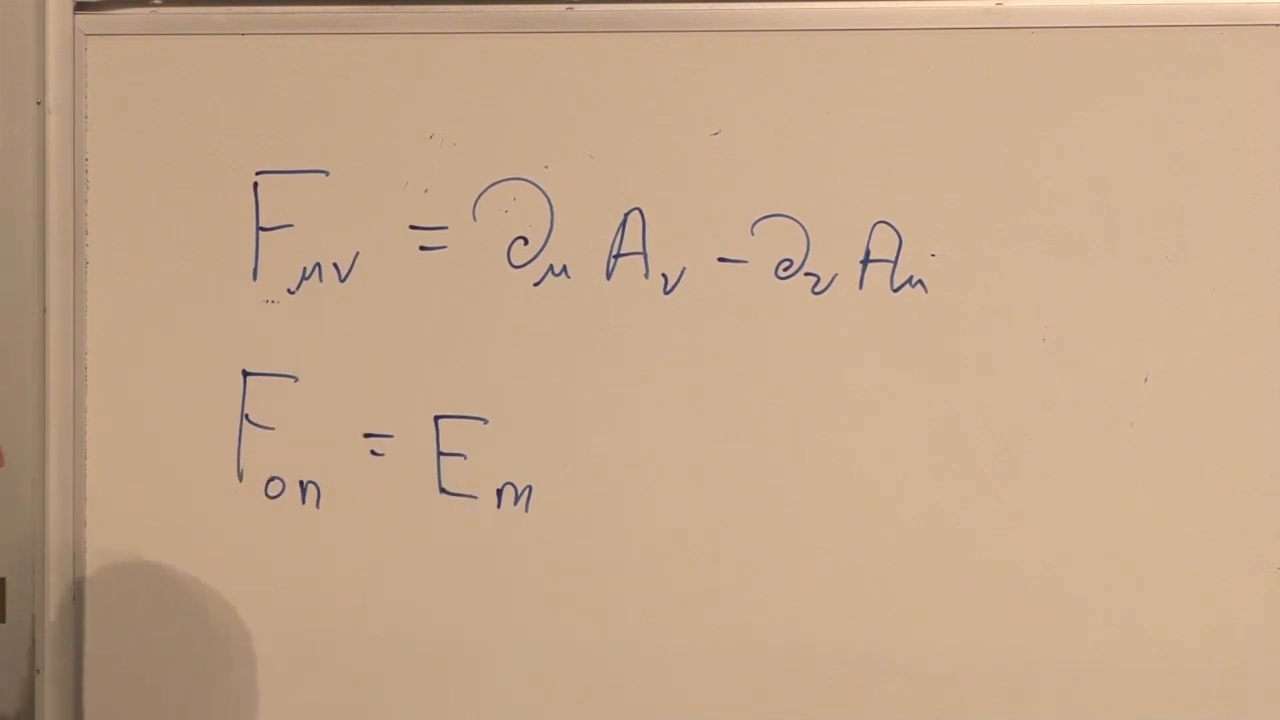
\includegraphics[width=\linewidth]{lecture_08_figure_02.png}
\caption{Định nghĩa tenxơ trường và thành phần hỗn hợp thời gian--không gian được đồng nhất với điện trường.}
\par\smallskip
\textit{Khung hình bài giảng: 00:13:15.}
\end{figure}

Quan hệ từ là phần không gian của cùng định nghĩa ấy. Chẳng hạn,
\begin{equation}
B_x
=
\partial_yA_z-\partial_zA_y
=
F_{yz},
\end{equation}
trong đó hai thành phần còn lại thu được bằng hoán vị vòng.

\begin{figure}[H]
\centering
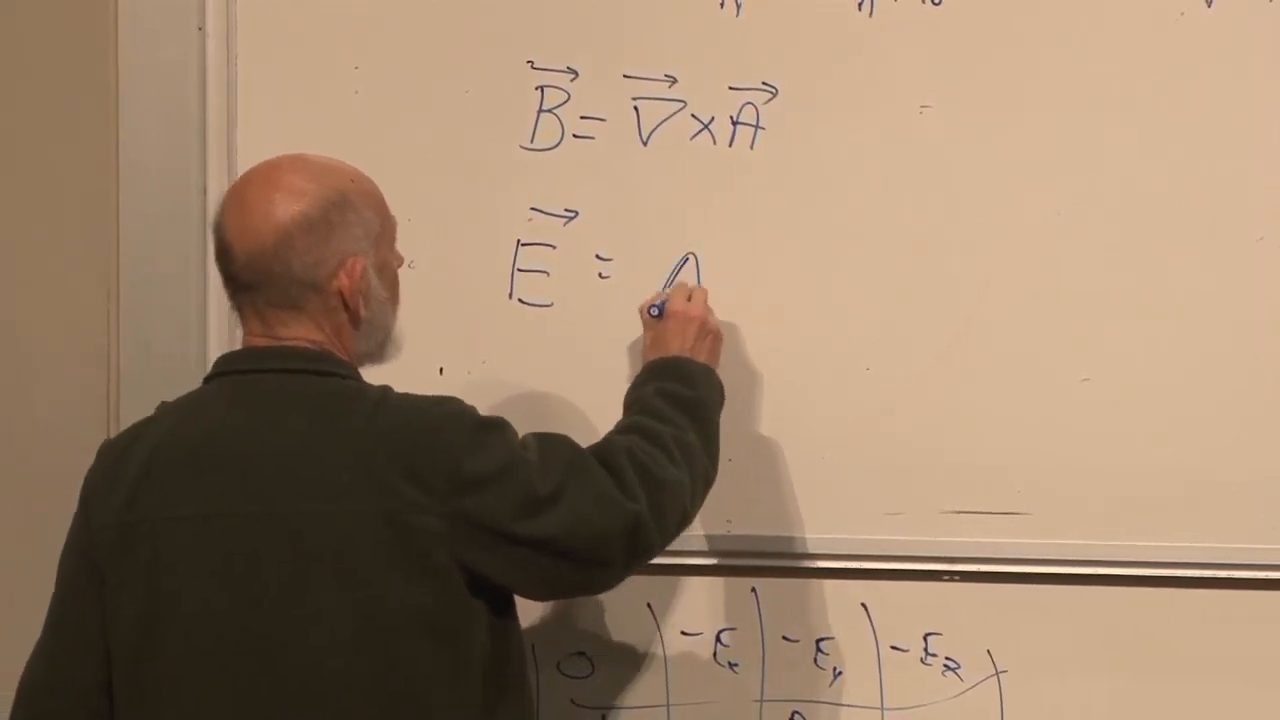
\includegraphics[width=\linewidth]{lecture_08_figure_03.png}
\caption{Các công thức thế vectơ cho điện trường và biểu thức xoáy cho từ trường được ghép lại trên bảng.}
\par\smallskip
\textit{Khung hình bài giảng: 00:14:00.}
\end{figure}

\subsection{Bảng các thành phần}

Hãy để chỉ số tenxơ thứ nhất gắn với các hàng và chỉ số thứ hai gắn với các cột, được sắp theo thứ tự \(0,x,y,z\). Khi đó
\begin{equation}
F_{\mu\nu}
=
\begin{pmatrix}
0&E_x&E_y&E_z\\
-E_x&0&B_z&-B_y\\
-E_y&-B_z&0&B_x\\
-E_z&B_y&-B_x&0
\end{pmatrix}.
\label{eq:f-lower-matrix}
\end{equation}
Phần biên hỗn hợp thời gian--không gian chứa \(\mathbf E\); khối không gian \(3\times3\) chứa \(\mathbf B\). Tam giác dưới không phải là thông tin mới, vì nó là ảnh phản chiếu đổi dấu của tam giác trên.

\begin{figure}[H]
\centering
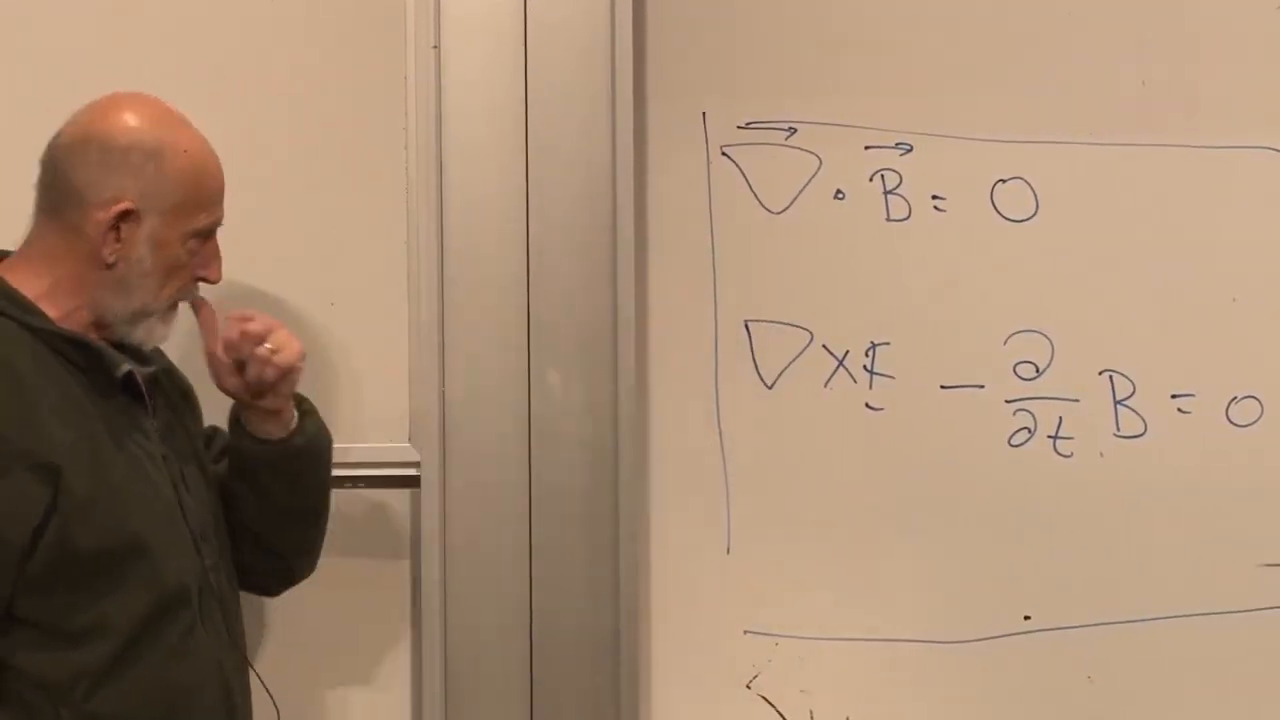
\includegraphics[width=\linewidth]{lecture_08_figure_04.png}
\caption{Tenxơ điện từ chỉ số dưới hoàn chỉnh, với biên điện và khối không gian từ trường của nó.}
\par\smallskip
\textit{Khung hình bài giảng: 00:17:15.}
\end{figure}

Nâng cả hai chỉ số làm đổi dấu mọi phần tử điện và giữ nguyên các phần tử từ:
\begin{equation}
F^{\mu\nu}
=
\begin{pmatrix}
0&-E_x&-E_y&-E_z\\
E_x&0&B_z&-B_y\\
E_y&-B_z&0&B_x\\
E_z&B_y&-B_x&0
\end{pmatrix}.
\label{eq:f-upper-matrix}
\end{equation}
Một thành phần điện mang một chỉ số thời gian và vì thế nhận một dấu trừ. Một thành phần từ mang hai chỉ số không gian và không nhận dấu nào.

\begin{classroomqa}
\audiencequestion{Tôi đọc ma trận như vậy có đúng không: các thành phần từ không có chỉ số thời gian?}
\lecturerresponse{Đúng. Chúng nằm trong khối thuần không gian. Các thành phần điện chính là các phần tử hỗn hợp thời gian--không gian dọc theo hàng đầu tiên và cột đầu tiên. \lecturetimestamp{00:18:55}}
\end{classroomqa}

\section{Biến đổi boost của một từ trường thuần túy}

Xét một phép boost dọc theo \(x\), với \(c=1\):
\begin{align}
t'&=\gamma(t-vx),
&
x'&=\gamma(x-vt),
&
y'&=y,
&
z'&=z,
\end{align}
trong đó
\begin{equation}
\gamma=\frac{1}{\sqrt{1-v^2}}.
\end{equation}
Ở dạng ma trận,
\begin{equation}
x'^\mu
=
\Lambda^\mu{}_\nu x^\nu,
\qquad
\Lambda^\mu{}_\nu
=
\begin{pmatrix}
\gamma&-\gamma v&0&0\\
-\gamma v&\gamma&0&0\\
0&0&1&0\\
0&0&0&1
\end{pmatrix}.
\label{eq:x-boost}
\end{equation}

\begin{classroomqa}
\audiencequestion{Có thiếu một dấu trừ trong ma trận boost không?}
\lecturerresponse{Có. Các phần tử ngoài đường chéo thời gian--không gian mang các dấu trừ cần thiết theo \(t'=\gamma(t-vx)\) và
\(x'=\gamma(x-vt)\). Sự hiệu chỉnh được thực hiện trước khi dùng phép biến đổi trường. \lecturetimestamp{00:23:50}}
\end{classroomqa}

\begin{figure}[H]
\centering
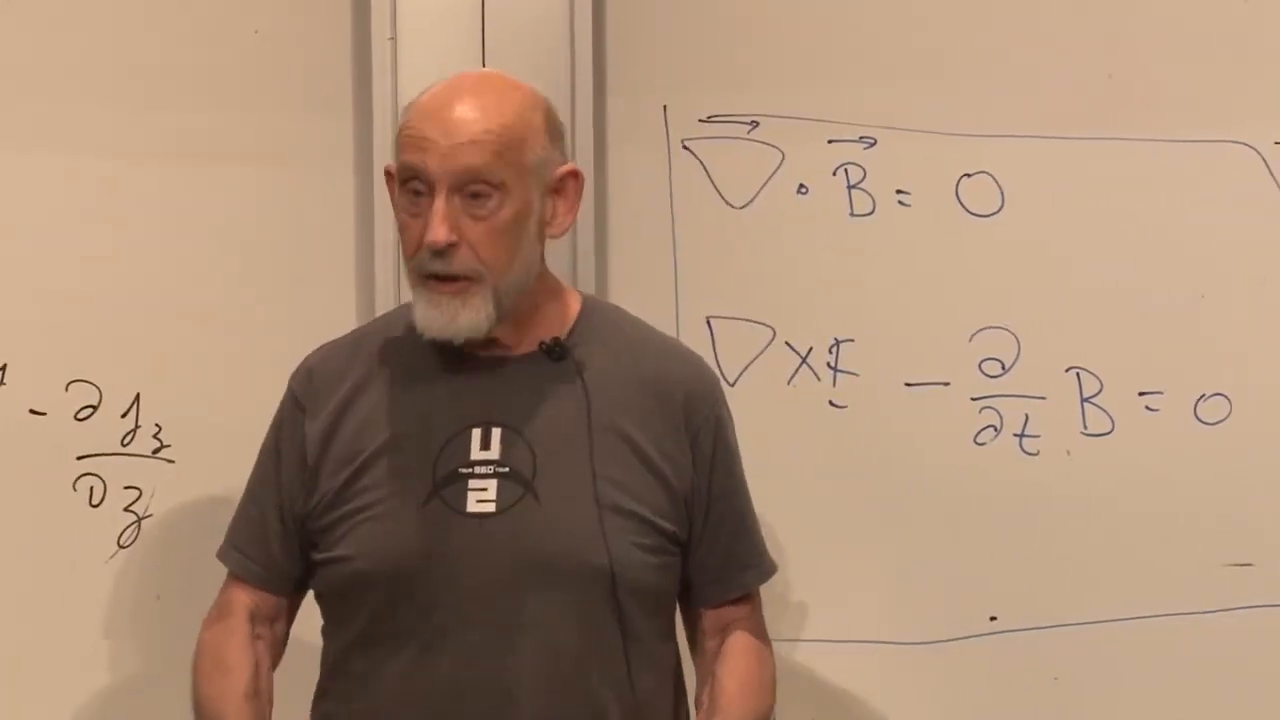
\includegraphics[width=\linewidth]{lecture_08_figure_05.png}
\caption{Ma trận boost Lorentz đã hiệu chỉnh cho chuyển động dọc theo trục \(x\).}
\par\smallskip
\textit{Khung hình bài giảng: 00:24:00.}
\end{figure}

Mỗi chỉ số trên của tenxơ biến đổi như một chỉ số trên của vectơ. Vì vậy
\begin{equation}
F'^{\mu\nu}
=
\Lambda^\mu{}_\sigma
\Lambda^\nu{}_\tau
F^{\sigma\tau}.
\label{eq:f-boost-law}
\end{equation}
Các \(\sigma\) và \(\tau\) lặp lại là các chỉ số giả. Với một tenxơ có nhiều chỉ số hơn, sẽ xuất hiện một ma trận biến đổi cho mỗi chỉ số.

\begin{figure}[H]
\centering
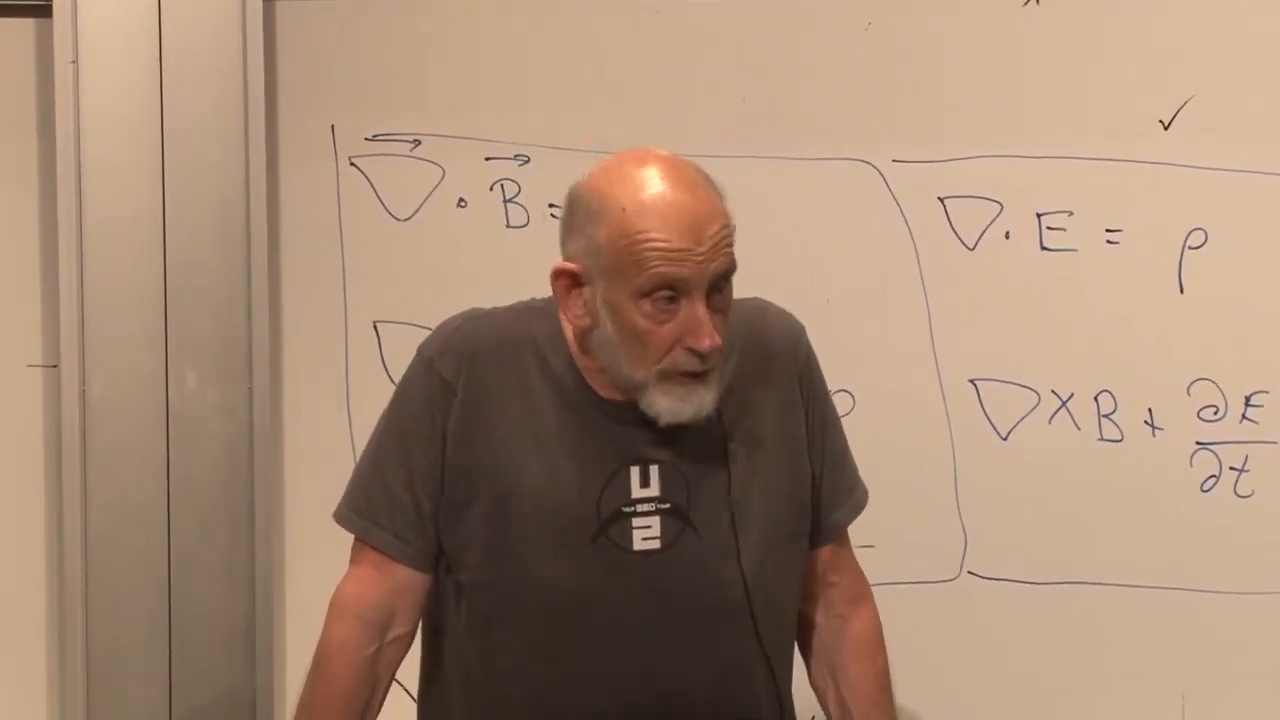
\includegraphics[width=\linewidth]{lecture_08_figure_06.png}
\caption{Quy luật biến đổi Lorentz hạng hai, với một ma trận boost cho mỗi chỉ số của tenxơ trường.}
\par\smallskip
\textit{Khung hình bài giảng: 00:26:40.}
\end{figure}

\subsection{Thành phần trở thành thành phần điện}

Giả sử hệ không phẩy chỉ chứa một từ trường \(B_y\). Theo các quy ước của Phương trình~\eqref{eq:f-upper-matrix}, thành phần độc lập liên quan là
\begin{equation}
F^{xz}=-B_y.
\end{equation}
Ta tìm thành phần hỗn hợp có phẩy \(F'^{0z}\), vì nó mang thành phần \(z\) có phẩy của điện trường. Phương trình
\eqref{eq:f-boost-law} cho
\begin{align}
F'^{0z}
&=
\Lambda^0{}_\sigma
\Lambda^z{}_\tau F^{\sigma\tau}
\\
&=
\Lambda^0{}_x\Lambda^z{}_zF^{xz}
\\
&=
(-\gamma v)(1)(-B_y)
=
\gamma vB_y.
\end{align}
Vì trong quy ước này \(F'^{0z}=-E'_z\),
\begin{equation}
E'_z=-\gamma vB_y.
\label{eq:boosted-electric-field}
\end{equation}
Dấu phụ thuộc vào các quy ước đã chọn về trục và trường; điểm bất biến của phép tính là
\begin{equation}
\lvert E'_z\rvert
=
\gamma\lvert vB_y\rvert
\ne0.
\end{equation}
Tổng kép co lại vì trường ban đầu chỉ có đúng một thành phần từ độc lập này.

\begin{figure}[H]
\centering
\includegraphics[width=\linewidth]{lecture_08_figure_07.png}
\caption{Thành phần tenxơ được chọn sau phép boost, cho thấy thừa số \(\gamma v\) nhân với thành phần từ ban đầu.}
\par\smallskip
\textit{Khung hình bài giảng: 00:32:30.}
\end{figure}

Hãy chọn hệ có phẩy chuyển động cùng điện tích. Khi đó điện tích đứng yên, nên trong lực tác dụng lên nó không còn phần từ \(q\,\mathbf v'\times\mathbf B'\). Thế nhưng lực không biến mất: nó là \(q\mathbf E'\). Lực từ theo người quan sát trong phòng thí nghiệm và lực điện theo người quan sát cùng chuyển động là hai mô tả của cùng một sự kiện.

Đó là câu trả lời cho câu đố trong đoạn văn đầu tiên của Einstein. Câu hỏi ấy chiếm chừng bốn mươi phút đầu của bài giảng này; câu đùa mang tính lịch sử là nó đã chiếm Einstein lâu hơn nhiều. Phép tính này đáng với thời gian bỏ ra vì nó biến khẩu hiệu rằng điện trường và từ trường trộn lẫn vào nhau thành một thành phần tenxơ tường minh.

\section{Phương trình Maxwell: đồng nhất thức và động lực học}

Bây giờ ta chuyển từ lực tác dụng lên điện tích sang các phương trình trường. Chúng sẽ được suy ra từ một tác dụng trong bài giảng tiếp theo. Ở đây mục đích trước hết là phát biểu chúng, hiểu hai vai trò lôgic khác nhau của chúng, và đưa nửa dựa trên đồng nhất thức vào dạng hiệp biến.

\begin{classroomqa}
\audiencequestion{Chẳng phải chúng ta đã suy ra các phương trình này rồi sao?}
\lecturerresponse{Chúng ta đã suy ra phương trình chuyển động của một hạt mang điện trong một trường điện từ cho trước. Các phương trình Maxwell là các phương trình chuyển động của chính trường đó, bao gồm cả phản ứng của trường đối với điện tích và dòng điện. \lecturetimestamp{00:35:10}}
\end{classroomqa}

\begin{classroomqa}
\audiencequestion{Có bao nhiêu phương trình Maxwell?}
\lecturerresponse{Có tám phương trình thành phần vô hướng. Ký hiệu vectơ gói chúng thành hai phương trình vô hướng và hai phương trình vectơ ba thành phần, theo quy ước được gọi là bốn phương trình Maxwell.
\lecturetimestamp{00:35:24}}
\end{classroomqa}

Ta tiếp tục dùng đơn vị trong đó \(c=1\) và các hằng số chân không thông dụng đã được hấp thụ vào định nghĩa của điện tích và dòng điện. Bốn trong tám phương trình thành phần suy ra từ định nghĩa \(F=dA\). Chúng là các đồng nhất thức động học. Bốn phương trình còn lại là động lực học và có thể thay đổi nếu tác dụng của trường thay đổi.

\subsection{Ba phép toán vectơ cơ bản}

Với một trường vectơ ba chiều khả vi \(\mathbf A\),
\begin{align}
(\boldsymbol\nabla\times\mathbf A)_x
&=
\partial_yA_z-\partial_zA_y,
\\
\boldsymbol\nabla\cdot\mathbf A
&=
\partial_xA_x+\partial_yA_y+\partial_zA_z.
\end{align}
Các thành phần xoáy còn lại thu được bằng cách hoán vị vòng \(x\to y\to z\to x\). Với một trường vô hướng \(s\),
\begin{equation}
\boldsymbol\nabla s
=
(\partial_xs,\partial_ys,\partial_zs).
\end{equation}
Vì vậy, xoáy là một vectơ, phân kỳ là một vô hướng, còn gradient là một vectơ.

\begin{classroomqa}
\audiencequestion{Có ai cần ôn lại đầy đủ các định nghĩa của xoáy và phân kỳ không?}
\lecturerresponse{Các định nghĩa theo thành phần đã được ghi lại, nhưng không cần khai triển hết mọi thành phần còn lại. Chỉ cần quay vòng các nhãn tọa độ là thu được chúng. \lecturetimestamp{00:37:32}}
\end{classroomqa}

Tính giao hoán của các đạo hàm riêng trơn kéo theo hai đồng nhất thức:
\begin{align}
\boldsymbol\nabla\cdot
(\boldsymbol\nabla\times\mathbf A)
&=0,
\label{eq:div-curl}
\\
\boldsymbol\nabla\times
(\boldsymbol\nabla s)
&=\mathbf0.
\label{eq:curl-grad}
\end{align}

\begin{classroomqa}
\audiencequestion{Có nên viết ra đầy đủ chứng minh theo thành phần rằng phân kỳ của xoáy bằng không không?}
\lecturerresponse{Cả lớp từ chối. Khai triển các thành phần sẽ tạo ra những cặp như \(\partial_x\partial_yA_z\) và
\(-\partial_y\partial_xA_z\), chúng triệt tiêu nhau vì có thể đổi chỗ thứ tự đạo hàm. \lecturetimestamp{00:40:13}}
\end{classroomqa}

\begin{figure}[H]
\centering
\includegraphics[width=\linewidth]{lecture_08_figure_08.png}
\caption{Các đồng nhất thức phân kỳ-của-xoáy và xoáy-của-gradient được dùng để thu được một nửa các phương trình Maxwell.}
\par\smallskip
\textit{Khung hình bài giảng: 00:41:40.}
\end{figure}

\subsection{Không có nguồn từ xuất phát từ thế vectơ}

Lấy phân kỳ của Phương trình~\eqref{eq:b-from-a} cho
\begin{equation}
\boldsymbol\nabla\cdot\mathbf B
=
\boldsymbol\nabla\cdot
(\boldsymbol\nabla\times\mathbf A)
=0.
\label{eq:div-b-zero}
\end{equation}
Không hề dùng phương trình chuyển động nào. Kết quả này chỉ theo từ mô tả bằng thế và các đạo hàm trơn.

\begin{figure}[H]
\centering
\includegraphics[width=\linewidth]{lecture_08_figure_09.png}
\caption{Độ phân kỳ của từ trường được quy về độ phân kỳ của một xoáy.}
\par\smallskip
\textit{Khung hình bài giảng: 00:43:05.}
\end{figure}

\begin{classroomqa}
\audiencequestion{Độ phân kỳ của điện trường là gì?}
\lecturerresponse{Đó là mật độ điện tích trong hệ đơn vị đang dùng, \(\boldsymbol\nabla\cdot\mathbf E=\rho\). Điện tích điểm là nguyên mẫu của các đường sức điện tỏa ra từ một nguồn.
\lecturetimestamp{00:43:20}}
\end{classroomqa}

Ở mức sơ cấp này, Phương trình~\eqref{eq:div-b-zero} cho biết không có mật độ điện tích từ. Một thế vectơ trơn, xác định toàn cục không thể tạo ra một nguồn đơn cực từ. Về sau, phát biểu này cần được nói kèm sự dè dặt: có thể mô tả đơn cực bằng các thế được xác định trên những miền chồng lấp hoặc bằng các lựa chọn chuẩn kỳ dị. Bài giảng tạm hoãn sự tinh chỉnh đó.

\subsection{Phương trình Faraday từ thế điện}

Phương trình~\eqref{eq:e-from-a}, viết theo ký hiệu vectơ ba chiều, là
\begin{equation}
\mathbf E
=
\frac{\partial\mathbf A}{\partial t}
-\boldsymbol\nabla A_0.
\label{eq:e-vector-potential}
\end{equation}
Mặc dù \(A_0\) là thành phần của một bốn-vectơ, nó là một vô hướng dưới các phép quay không gian thông thường. Lấy xoáy:
\begin{align}
\boldsymbol\nabla\times\mathbf E
&=
\boldsymbol\nabla\times
\frac{\partial\mathbf A}{\partial t}
-
\boldsymbol\nabla\times
(\boldsymbol\nabla A_0)
\\
&=
\frac{\partial}{\partial t}
(\boldsymbol\nabla\times\mathbf A)
\\
&=
\frac{\partial\mathbf B}{\partial t}.
\end{align}
Phép xoáy theo không gian giao hoán với đạo hàm theo thời gian, còn xoáy của gradient thì triệt tiêu.

\begin{figure}[H]
\centering
\includegraphics[width=\linewidth]{lecture_08_figure_10.png}
\caption{Biểu thức xoáy của từ trường, công thức thế điện, và phần mở đầu của phép tính xoáy trong cùng một trạng thái bảng đã hoàn chỉnh.}
\par\smallskip
\textit{Khung hình bài giảng: 00:47:45.}
\end{figure}

Vì thế bốn phương trình thành phần thuần nhất là
\begin{align}
\boldsymbol\nabla\cdot\mathbf B&=0,
\label{eq:homogeneous-div}
\\
\boldsymbol\nabla\times\mathbf E
-\frac{\partial\mathbf B}{\partial t}
&=\mathbf0.
\label{eq:homogeneous-curl}
\end{align}
Phương trình thứ nhất là một phương trình vô hướng; phương trình thứ hai là một phương trình vectơ gồm ba thành phần.

\begin{figure}[H]
\centering
\includegraphics[width=\linewidth]{lecture_08_figure_11.png}
\caption{Cặp phương trình Maxwell không nguồn thu được trực tiếp từ các định nghĩa của thế.}
\par\smallskip
\textit{Khung hình bài giảng: 00:48:45.}
\end{figure}

\subsection{Nửa động lực học}

Các phương trình còn lại là
\begin{align}
\boldsymbol\nabla\cdot\mathbf E&=\rho,
\label{eq:gauss-electric}
\\
\boldsymbol\nabla\times\mathbf B
+\frac{\partial\mathbf E}{\partial t}
&=-\mathbf J.
\label{eq:ampere-maxwell}
\end{align}
Chúng không phải là hệ quả của \(F=dA\). Chúng mô tả cách các nguồn tạo ra và làm biến đổi trường, và bài giảng tiếp theo sẽ suy ra chúng từ tác dụng điện từ. Dấu trừ trước dòng điện được cố định bởi các quy ước đã chọn trước đó: \(F_{0i}=E_i\),
\(F_{ij}=\epsilon_{ijk}B_k\), và
\(\partial_\mu F^{\mu\nu}=J^\nu\). Trên bảng giảng trực tiếp, ban đầu \(\mathbf J\) được đặt ở vế phải mà không có dấu trừ này; sự không khớp do đó với bảo toàn điện tích được nhận ra và được sửa trong bài giảng tiếp theo.

\begin{classroomqa}
\audiencequestion{Đại lượng ở vế phải của phương trình xoáy là loại đại lượng gì?}
\lecturerresponse{Vế trái là một vectơ ba chiều, nên vế phải là một vectơ ba chiều gọi là mật độ dòng điện \(\mathbf J\). Vế phải của phương trình Gauss là mật độ điện tích vô hướng ba chiều \(\rho\).
\lecturetimestamp{00:50:36}}
\end{classroomqa}

\begin{figure}[H]
\centering
\includegraphics[width=\linewidth]{lecture_08_figure_12.png}
\caption{Bốn phương trình Maxwell được nhóm thành cặp dựa trên đồng nhất thức và cặp động lực học có nguồn.}
\par\smallskip
\textit{Khung hình bài giảng: 00:50:40.}
\end{figure}

\section{Điện tích và dòng điện như dòng chảy trong không-thời gian}

Các ký hiệu \(\rho\) và \(\mathbf J\) giờ phải được gán ý nghĩa hình học. Mật độ điện tích là điện tích trên một đơn vị thể tích; mật độ dòng điện là điện tích đi qua một diện tích có định hướng trong một đơn vị thời gian. Bài giảng phát triển cả hai từ các đường thế giới để sự hợp nhất sau này của chúng thành một bốn-vectơ sẽ không có vẻ ngẫu nhiên.

\subsection{Một lời bình bên lề trong lớp từ tấm bảng ở phòng bên}

Trước khi vẽ các đường thế giới ấy, những phương trình nhìn thấy ở phòng bên dẫn tới một đoạn bình bên lề ngắn về giảng dạy. Một môn học sắp tới sẽ giới thiệu cơ học lượng tử cho các giảng viên toán muốn có nền tảng cần thiết cho lý thuyết trường lượng tử và các liên hệ của nó với toán học hiện đại. Thách thức diễn ra theo cả hai chiều: nhà vật lý phải làm tường minh những thói quen vật lý vốn ngầm định, còn nhà toán học phải học xem các cấu trúc hình thức ấy đang được yêu cầu mô tả điều gì.

\begin{classroomqa}
\audiencequestion{Ai được cho là sẽ thấy phân công giảng dạy đó gây nản lòng?}
\lecturerresponse{Có thể là cả hai phía: các nhà vật lý giảng cho một cử tọa không quen thuộc và các nhà toán học đối mặt với những thói quen vật lý nằm sau hình thức luận. Tuy vậy, công việc ấy vẫn được kỳ vọng là thú vị. Sau đó lớp quay lại với điện tích và dòng điện. \lecturetimestamp{00:53:20}}
\end{classroomqa}

\subsection{Mật độ điện tích}

Hãy vẽ thời gian theo phương thẳng đứng và để các hướng còn lại được vẽ đại diện cho không gian ba chiều. Các hạt mang điện vạch ra các đường thế giới. Tại một thời điểm cố định, đặt một khối lập phương không gian nhỏ có thể tích \(\Delta V\) cắt qua bó đường thế giới đó và cộng các điện tích của các hạt bên trong nó. Mật độ điện tích là
\begin{equation}
\rho(t,\mathbf x)
=
\lim_{\Delta V\to0}
\frac{\Delta Q}{\Delta V}.
\label{eq:charge-density}
\end{equation}
Hình vuông hai chiều trên bảng biểu diễn một khối lập phương ba chiều; hướng không gian bị thiếu chỉ bị lược bỏ vì không thể vẽ bốn chiều trên một tấm bảng phẳng.

\begin{figure}[H]
\centering
\includegraphics[width=\linewidth]{lecture_08_figure_13.png}
\caption{Các đường thế giới của hạt mang điện cắt qua một ô không gian nhỏ, với \(\rho=\Delta Q/\Delta V\).}
\par\smallskip
\textit{Khung hình bài giảng: 00:57:20.}
\end{figure}

\subsection{Mật độ dòng điện}

Lật ô không-thời gian sang một bên. Để định nghĩa \(J_x\), hãy chọn một cửa sổ nhỏ có diện tích \(\Delta A_x\) trong mặt phẳng \(yz\), vuông góc với trục \(x\). Đếm điện tích thuần đi qua từ phía \(x\) âm sang phía \(x\) dương trong \(\Delta t\):
\begin{equation}
J_x
=
\lim_{\Delta A_x,\Delta t\to0}
\frac{\Delta Q_x}{\Delta A_x\,\Delta t}.
\label{eq:jx-window}
\end{equation}
Hướng định hướng quyết định dấu. Các cửa sổ vuông góc với \(y\) và \(z\) định nghĩa \(J_y\) và \(J_z\) theo cùng cách.

Bản vẽ trên bảng thành thật cho thấy sự khó khăn của việc minh họa: một cửa sổ trong mặt phẳng \(yz\) trông giống cửa sổ trên trần hơn là trên tường. Đơn giản là có nhiều trục liên quan hơn số trục có thể hiển thị cùng một lúc. Định nghĩa bất biến thì không mơ hồ ngay cả khi hình phác thảo không rõ ràng.

\begin{classroomqa}
\audiencequestion{Cửa sổ trong hình vẽ có ở trên trần không?}
\lecturerresponse{Theo phép ví von căn phòng thì có. Điều quan trọng là mặt phẳng của nó vuông góc với hướng \(x\). Một diện tích \(yz\) đo dòng theo hướng \(x\) đi qua nó. \lecturetimestamp{00:59:38}}
\end{classroomqa}

\begin{figure}[H]
\centering
\includegraphics[width=\linewidth]{lecture_08_figure_14.png}
\caption{Dòng điện tích qua một cửa sổ ngang, với \(J_x=\Delta Q/(\Delta A\,\Delta t)\).}
\par\smallskip
\textit{Khung hình bài giảng: 01:01:40.}
\end{figure}

\begin{figure}[H]
\centering
\includegraphics[width=\linewidth]{lecture_08_figure_15.png}
\caption{Ba thành phần dòng điện được xác định bởi điện tích đi qua các cửa sổ vuông góc với ba trục không gian.}
\par\smallskip
\textit{Khung hình bài giảng: 01:02:40.}
\end{figure}

Bốn đại lượng ấy có các định nghĩa song song. Một thể tích không gian tại một thời điểm là một siêu mặt vuông góc với trục thời gian, nên \(\rho\) là dòng điện tích qua một cửa sổ có pháp tuyến theo thời gian. Các \(J_i\) là các dòng qua những cửa sổ có pháp tuyến theo không gian.

\begin{classroomqa}
\audiencequestion{Bốn số ấy có phải là một dòng theo hướng thời gian và ba dòng theo các hướng không gian không?}
\lecturerresponse{Đó chính xác là hình dung hữu ích. Một thể tích không gian là một cửa sổ vuông góc với trục thời gian; ba diện tích ngang là các cửa sổ vuông góc với \(x\), \(y\), và \(z\). Bốn thông lượng ấy thuộc về cùng một nhóm. \lecturetimestamp{01:04:14}}
\end{classroomqa}

Điều này gợi ý tứ-dòng phản biến
\begin{equation}
J^\mu
=
(\rho,J_x,J_y,J_z).
\label{eq:four-current}
\end{equation}

\begin{classroomqa}
\audiencequestion{Metric xuất hiện ở đâu, và dòng này là hiệp biến hay phản biến?}
\lecturerresponse{Theo cách định nghĩa ở đây, \(\rho\) và ba \(J_i\) tạo thành các thành phần của \(J^\mu\), một bốn-vectơ chỉ số trên, hay phản biến. Metric hạ chỉ số của nó khi cần \(J_\mu\). Cách viết Maxwell hiệp biến sẽ cho thấy vì sao lựa chọn chỉ số trên là tự nhiên.
\lecturetimestamp{01:04:48}}
\end{classroomqa}

\section{Đoạn xen trong giờ nghỉ: tín hiệu gần một lỗ đen}

Đúng vào giờ nghỉ đã định, các câu hỏi chuyển sang một cuộc thảo luận trước đó về lỗ đen. Mặc dù đây là một sự lạc đề khỏi điện động lực học, đó là một trao đổi đáng kể trong lớp và minh họa cùng một kỷ luật là tách biệt các mô tả do những quan sát viên khác nhau đưa ra.

\begin{classroomqa}
\audiencequestion{Nếu một quan sát viên ở xa thấy một vật đang rơi chậm lại gần chân trời, thì lỗ đen có nên trông như bị phủ kín bởi mọi thứ từng rơi vào nó không?}
\lecturerresponse{Trong thời gian tọa độ Schwarzschild, sự rơi vào cổ điển được thấy là tiến gần chân trời một cách tiệm cận. Có thể hình dung vật chất đến sau như những lớp ngày càng bị nén gần chân trời. Tuy nhiên, về mặt thao tác, tín hiệu đi ra ngày càng bị trễ, bị dịch đỏ và yếu đi. Ánh sáng phát ra ở một tần số cục bộ thông thường đến trước hết dưới dạng ánh sáng quang học, rồi hồng ngoại, vi ba và vô tuyến, với mỗi photon mang ít năng lượng hơn. Không có máy dò ở xa nào thực tế cứ tiếp tục thấy một vật sáng bị đóng băng mãi mãi; nó mờ dần vào bóng tối.
\lecturetimestamp{01:06:11}}
\end{classroomqa}

Đồng hồ của người quan sát đang rơi vào và chiếc đèn pin phát ra cục bộ của người đó vẫn là những thứ bình thường đối với chính họ. Mô tả từ xa khác đi vì tần số và tốc độ đến đều bị dịch đỏ. Với năng lượng hữu hạn và băng thông hữu hạn, trên thực tế sẽ có một phần cuối cùng của thông điệp còn phân giải được.

\begin{classroomqa}
\audiencequestion{Vật đó có đang tiến gần tiệm cận tới chân trời sự kiện không?}
\lecturerresponse{Đó là mô tả từ xa trong tọa độ Schwarzschild. Về mặt lượng tử, tín hiệu mờ dần ấy cũng phải được phân biệt với bức xạ Hawking của lỗ đen. Ở những thời điểm đủ muộn, tín hiệu dịch đỏ yếu ấy về mặt quan sát bị chìm mất trong nền bức xạ của chính lỗ đen. \lecturetimestamp{01:09:24}}
\end{classroomqa}

\begin{classroomqa}
\audiencequestion{Điều gì xảy ra nếu bước sóng bị dịch đỏ tăng vượt quá thang đo của vũ trụ quan sát được?}
\lecturerresponse{Tín hiệu trên thực tế bị mất từ lâu trước giới hạn đó. Bài giảng đưa ra bức tranh Hawking theo bậc độ lớn, với cỡ một lượng tử điển hình cho mỗi thời gian ánh sáng băng qua,
\[
t_{\rm cross}\sim\frac{R_s}{c}.
\]
Đối với một lỗ lớn, đây là bức xạ cực kỳ yếu, và một tín hiệu rơi vào bị dịch đỏ đủ mạnh sẽ trở nên không thể phát hiện sớm hơn nhiều so với bất kỳ giới hạn bước sóng vũ trụ học nào. \lecturetimestamp{01:09:50}}
\end{classroomqa}

\begin{classroomqa}
\audiencequestion{Tốc độ cỡ một lượng tử trên mỗi thời gian băng qua có giữ cố định trong suốt đời của lỗ đen không?}
\lecturerresponse{Không. Một lỗ đen Schwarzschild đang bay hơi co lại, nên thời gian băng qua của nó giảm và nhiệt độ Hawking của nó tăng. Vì thế sự phát xạ tăng tốc. Ước lượng theo thứ nguyên theo bán kính tức thời vẫn hữu ích, nhưng bán kính không hằng. Tương ứng, bước sóng Hawking điển hình ngắn lại khi sự bay hơi tiến triển. \lecturetimestamp{01:11:42}}
\end{classroomqa}

Sau giờ nghỉ, khi áo khoác đã được cởi ra, ta quay lại \(\rho\) và \(\mathbf J\).

\section{Bảo toàn điện tích cục bộ}

Thật dễ chỉ phát biểu bảo toàn điện tích dưới dạng
\begin{equation}
\frac{dQ_{\rm universe}}{dt}=0.
\end{equation}
Phát biểu đó quá yếu. Điện tích có thể biến mất khỏi một phòng thí nghiệm và xuất hiện lại tức thì ở Alpha Centauri, hoặc xa hơn trong Cụm Coma, mà không làm thay đổi tổng lượng. Một định luật như vậy sẽ có rất ít sức nặng thực nghiệm.

Phát biểu mạnh hơn là cục bộ: điện tích bên trong một vùng chỉ có thể thay đổi bằng cách đi qua biên của vùng đó. Hãy đặt một hộp nhỏ quanh một điểm. Nếu điện tích của nó tăng, phải có một dòng thuần đi vào qua sáu mặt của hộp; nếu nó giảm, phải có một dòng thuần đi ra.

\subsection{Thông lượng qua các mặt đối diện}

Xét hai mặt vuông góc với \(x\). Đóng góp hướng vào trên một mặt được tính tại một giá trị của \(x\); đóng góp trên mặt đối diện được tính ở một điểm cách đó một khoảng nhỏ. Hiệu của chúng, chia cho bề rộng của hộp, tiến tới
\begin{equation}
-\partial_xJ_x.
\end{equation}
Dấu trừ xuất hiện vì \(J_x\) dương được định nghĩa là dòng chảy theo chiều \(x\) tăng, trong khi một thông lượng đi ra làm giảm điện tích trong hộp. Các cặp mặt vuông góc với \(y\) và \(z\) cũng lần lượt đóng góp \(-\partial_yJ_y\) và \(-\partial_zJ_z\). Do đó
\begin{equation}
\frac{\partial\rho}{\partial t}
=
-\partial_xJ_x-\partial_yJ_y-\partial_zJ_z
=
-\boldsymbol\nabla\cdot\mathbf J.
\end{equation}
Tương đương,
\begin{equation}
\boxed{
\frac{\partial\rho}{\partial t}
+\boldsymbol\nabla\cdot\mathbf J=0
}.
\label{eq:continuity}
\end{equation}

\begin{figure}[H]
\centering
\includegraphics[width=\linewidth]{lecture_08_figure_16.png}
\caption{Định luật cân bằng cục bộ
\(\dot\rho=-\boldsymbol\nabla\cdot\mathbf J\), cùng với hộp nhỏ mà các dòng qua biên của nó tạo ra hệ thức ấy.}
\par\smallskip
\textit{Khung hình bài giảng: 01:20:45.}
\end{figure}

Điều này theo quy ước được gọi là phương trình liên tục. Bài giảng chuộng tên \emph{bảo toàn địa phương} hơn: chữ liên tục có thể gợi ra một giả thiết trơn toán học, trong khi nội dung vật lý là điện tích không thể biến mất ở đây rồi xuất hiện lại ở kia mà không có một dòng điện ở giữa.

\subsection{Vì sao Maxwell cần dòng điện dịch}

Phương trình~\eqref{eq:continuity} không phải là một bổ sung độc lập vào các phương trình Maxwell. Lấy đạo hàm theo thời gian của định luật Gauss và lấy phân kỳ của định luật Ampère--Maxwell:
\begin{align}
\frac{\partial\rho}{\partial t}
&=
\boldsymbol\nabla\cdot
\frac{\partial\mathbf E}{\partial t},
\\
-\boldsymbol\nabla\cdot\mathbf J
&=
\boldsymbol\nabla\cdot
(\boldsymbol\nabla\times\mathbf B)
+
\boldsymbol\nabla\cdot
\frac{\partial\mathbf E}{\partial t}
\\
&=
\boldsymbol\nabla\cdot
\frac{\partial\mathbf E}{\partial t}.
\end{align}
Vì thế hai vế trái bằng nhau, suy ra
\(\partial_t\rho=-\boldsymbol\nabla\cdot\mathbf J\), đúng bằng
Phương trình~\eqref{eq:continuity}. Điều quan trọng về mặt cấu trúc là đạo hàm theo thời gian của \(\mathbf E\), tức hạng dòng điện dịch, là thiết yếu để quan hệ phân kỳ tương thích với bảo toàn điện tích.

\begin{classroomqa}
\audiencequestion{Ta vẫn chưa chỉ ra hai phương trình Maxwell có nguồn xuất phát từ đâu, phải không?}
\lecturerresponse{Chưa. Chúng là mục tiêu động lực học và sẽ được suy ra từ tác dụng vào buổi tới. Định luật xoáy tĩnh từ đã được biết đến trước Maxwell; phần bổ sung phụ thuộc thời gian mang tính quyết định của ông là dòng điện dịch. Sự hiện diện của nó khiến phương trình trường tương thích với bảo toàn điện tích địa phương. \lecturetimestamp{01:23:15}}
\end{classroomqa}

Phép tính phân kỳ chi tiết được để lại như một bài tập trong bài giảng, nhưng kết luận của nó không phải là tùy chọn: các phương trình Maxwell đòi hỏi sự bảo toàn điện tích.

\section{Tứ-dòng và phân kỳ của nó}

Viết Phương trình~\eqref{eq:continuity} theo các thành phần:
\begin{equation}
\frac{\partial\rho}{\partial t}
+
\frac{\partial J_x}{\partial x}
+
\frac{\partial J_y}{\partial y}
+
\frac{\partial J_z}{\partial z}
=0.
\label{eq:continuity-components}
\end{equation}

\begin{figure}[H]
\centering
\includegraphics[width=\linewidth]{lecture_08_figure_17.png}
\caption{Bảo toàn điện tích địa phương được khai triển thành một đạo hàm theo thời gian và ba đạo hàm theo không gian.}
\par\smallskip
\textit{Khung hình bài giảng: 01:25:40.}
\end{figure}

Với \(J^\mu\) được định nghĩa bởi Phương trình~\eqref{eq:four-current}, bốn hạng tử đó là một phép co:
\begin{equation}
\boxed{\partial_\mu J^\mu=0}.
\label{eq:four-current-conservation}
\end{equation}
Chỉ số dưới của \(\partial_\mu\) co với chỉ số trên của
\(J^\mu\), nên kết quả là một vô hướng Lorentz. Cấu trúc cửa sổ hình học đã gợi ra quy luật biến đổi này: \(\rho\) và ba thành phần của dòng điện là bốn định hướng của cùng một thông lượng điện tích.

\begin{figure}[H]
\centering
\includegraphics[width=\linewidth]{lecture_08_figure_18.png}
\caption{Các thành phần \((\rho,J_x,J_y,J_z)\) được ghép thành \(J^\mu\)
và co với gradient bốn chiều.}
\par\smallskip
\textit{Khung hình bài giảng: 01:27:10.}
\end{figure}

\begin{classroomqa}
\audiencequestion{Khi nào đạo hàm theo thời gian của \(\rho\) lại trở thành đạo hàm riêng?}
\lecturerresponse{Nó đã là đạo hàm riêng ngay từ đầu. Ta giữ cố định hộp không gian và hỏi mật độ điện tích của nó thay đổi thế nào khi thời gian thay đổi. Ta không đi theo một quỹ đạo chuyển động, nên
\(\dot\rho\) ở đây có nghĩa là
\(\partial\rho/\partial t\) tại \(x,y,z\) cố định.
\lecturetimestamp{01:28:20}}
\end{classroomqa}

\section{Các phương trình thuần nhất dưới dạng hiệp biến}

Giờ đây ta đã có các đối tượng cần thiết:
\begin{itemize}
\item \(\mathbf E\) và \(\mathbf B\) là 6 thành phần độc lập
của tensor phản đối xứng \(F_{\mu\nu}\);
\item \(\rho\) và \(\mathbf J\) là 4 thành phần của \(J^\mu\);
\item bảo toàn địa phương là phương trình vô hướng
\(\partial_\mu J^\mu=0\).
\end{itemize}
Nhiệm vụ còn lại của buổi giảng này là viết cặp phương trình Maxwell thuần nhất, các Phương trình~\eqref{eq:homogeneous-div} và
\eqref{eq:homogeneous-curl}, thành một phương trình tensor.

\subsection{Đạo hàm chu trình}

Câu trả lời là
\begin{equation}
\boxed{
\partial_\sigma F_{\nu\tau}
+
\partial_\nu F_{\tau\sigma}
+
\partial_\tau F_{\sigma\nu}
=0
}.
\label{eq:bianchi}
\end{equation}
Ba hạng tử phân bố theo chu trình chỉ số đạo hàm và hai chỉ số của tensor trường. Cách này thường được viết tắt là
\begin{equation}
\partial_{[\sigma}F_{\nu\tau]}=0,
\end{equation}
trong đó dấu ngoặc vuông biểu thị phép phản đối xứng hóa.

\begin{figure}[H]
\centering
\includegraphics[width=\linewidth]{lecture_08_figure_19.png}
\caption{Phương trình ba chỉ số theo chu trình gói gọn các phương trình Maxwell thuần nhất.}
\par\smallskip
\textit{Khung hình bài giảng: 01:33:20.}
\end{figure}

\subsection{Cả ba chỉ số đều là không gian}

Lấy
\begin{equation}
(\sigma,\nu,\tau)=(x,y,z).
\end{equation}
Khi đó
\begin{align}
0
&=
\partial_xF_{yz}
+
\partial_yF_{zx}
+
\partial_zF_{xy}
\\
&=
\partial_xB_x+\partial_yB_y+\partial_zB_z
\\
&=
\boldsymbol\nabla\cdot\mathbf B.
\end{align}
Vì vậy, thành phần hoàn toàn không gian của
Phương trình~\eqref{eq:bianchi} chính xác là điều kiện phân kỳ của từ trường bằng không.

\begin{figure}[H]
\centering
\includegraphics[width=\linewidth]{lecture_08_figure_20.png}
\caption{Thành phần hoàn toàn không gian của đồng nhất thức chu trình rút gọn thành
\(\partial_xB_x+\partial_yB_y+\partial_zB_z=0\).}
\par\smallskip
\textit{Khung hình bài giảng: 01:35:30.}
\end{figure}

\subsection{Một chỉ số thời gian}

Chọn, chẳng hạn,
\begin{equation}
(\sigma,\nu,\tau)=(y,x,0).
\end{equation}
Khi đó Phương trình~\eqref{eq:bianchi} kết hợp hai đạo hàm theo không gian của các thành phần điện với một đạo hàm theo thời gian của một thành phần từ:
\begin{equation}
\partial_yF_{x0}
+
\partial_xF_{0y}
+
\partial_0F_{yx}
=0.
\end{equation}
Dùng ma trận trong Phương trình~\eqref{eq:f-lower-matrix}, đây là một thành phần của
\begin{equation}
\boldsymbol\nabla\times\mathbf E
-\frac{\partial\mathbf B}{\partial t}
=\mathbf0,
\end{equation}
với các dấu tương đối được cố định bởi tính phản đối xứng. Chọn các cặp chỉ số không gian khác sẽ cho hai thành phần xoáy còn lại.

\begin{figure}[H]
\centering
\includegraphics[width=\linewidth]{lecture_08_figure_21.png}
\caption{Việc kiểm tra một thành phần với một chỉ số thời gian và hai chỉ số không gian, cho ra một thành phần của phương trình Faraday.}
\par\smallskip
\textit{Khung hình bài giảng: 01:38:20.}
\end{figure}

Cũng có một chứng minh trực tiếp. Thế Phương trình~\eqref{eq:field-tensor-definition} vào
Phương trình~\eqref{eq:bianchi}. Sáu hạng tử đạo hàm bậc hai xuất hiện, và chúng triệt tiêu từng cặp vì các đạo hàm riêng giao hoán. Đây là phiên bản bốn chiều của các đồng nhất thức phân kỳ của xoáy và xoáy của gradient.

\begin{classroomqa}
\audiencequestion{Trong tên Bianchi có \(h\) không?}
\lecturerresponse{Có. Phương trình chu trình là đồng nhất thức Bianchi điện từ, một trường hợp đặc biệt của một đồng nhất thức hình học cũng xuất hiện trong thuyết tương đối rộng. Cách diễn giải hình học sâu hơn của nó được hoãn lại.
\lecturetimestamp{01:40:28}}
\end{classroomqa}

\subsection{Vì sao 64 thành phần được viết ra chỉ chứa 4 phương trình}

Ba chỉ số, mỗi chỉ số có 4 giá trị khả dĩ, thoạt nhìn cho ra
\(4^3=64\) phương trình. Tính phản đối xứng loại bỏ sự dư thừa:
\begin{itemize}
\item nếu có bất kỳ hai chỉ số nào trùng nhau, biểu thức chu trình triệt tiêu đồng nhất;
\item nếu cả ba chỉ số đều khác nhau, các hoán vị tái tạo cùng một phương trình sai khác chỉ ở dấu;
\item trong bốn chiều chỉ có
\(\binom{4}{3}=4\) bộ ba không có thứ tự gồm các chỉ số khác nhau.
\end{itemize}
Có \(24\) bộ ba có thứ tự mà mọi chỉ số đều khác nhau, được gom thành bốn nhóm, mỗi nhóm gồm sáu hoán vị. \(40\) bộ ba có thứ tự còn lại thì triệt tiêu. Bốn phương trình độc lập là một phương trình phân kỳ từ và ba thành phần của phương trình Faraday.

\begin{classroomqa}
\audiencequestion{Tensor trường có 6 phần tử độc lập, nhưng biểu thức ba chỉ số dường như chứa 64 phương trình. Vì sao chỉ còn lại 4?}
\lecturerresponse{Các chỉ số lặp lại cho ra 0, còn các hoán vị của ba chỉ số khác nhau thì lặp lại cùng một hệ thức, chỉ khác dấu. Vì thế, 64 thành phần bề ngoài ấy sụp xuống còn 4 phương trình độc lập.
\lecturetimestamp{01:41:58}}
\end{classroomqa}

Phương trình~\eqref{eq:bianchi} hiển nhiên có tính tensor và vì thế hiệp biến Lorentz. Trong mô tả trơn bằng một thế duy nhất, nó cũng phát biểu rằng không có cả mật độ điện tích từ lẫn dòng điện từ. Cặp phương trình có nguồn mang tính động lực học được để đúng ở ranh giới mà bài giảng đã đi tới: phương trình hiệp biến của nó và phép suy ra từ tác dụng thuộc về buổi gặp tiếp theo.

\section{Đối ngẫu và câu hỏi về đơn cực}

Các câu hỏi cuối cùng quay trở lại sự bất đối xứng bề ngoài giữa nguồn điện và nguồn từ. Trong không gian rỗng, các phương trình Maxwell có phép quay đối ngẫu điện--từ
\begin{equation}
\mathbf E\longrightarrow\mathbf B,
\qquad
\mathbf B\longrightarrow-\mathbf E.
\label{eq:duality-quarter-turn}
\end{equation}
Đây là một phép quay 90 độ trong một mặt phẳng trừu tượng có các trục
\(\mathbf E\) và \(\mathbf B\), chứ không phải một phép phản xạ chỉ đơn thuần hoán đổi nhãn của chúng. Khi đồng thời có cả nguồn điện lẫn nguồn từ, tứ-dòng điện và tứ-dòng từ cũng phải quay cùng lúc.

\begin{figure}[H]
\centering
\includegraphics[width=\linewidth]{lecture_08_figure_22.png}
\caption{Hình ảnh kết thúc về đối ngẫu điện--từ: một góc quay một phần tư vòng trong
mặt phẳng \(E\)-\(B\) chứ không phải một sự hoán đổi đơn giản.}
\par\smallskip
\textit{Khung hình bài giảng: 01:45:00.}
\end{figure}

\begin{classroomqa}
\audiencequestion{Nếu các phương trình không nguồn là đối ngẫu dưới phép hoán đổi điện và từ, vì sao các thành phần điện lại là các phần tử thời gian--không gian còn các thành phần từ lại là các phần tử không gian--không gian?}
\lecturerresponse{Sự phân biệt đó phụ thuộc hệ quy chiếu trong
\(F_{\mu\nu}\), và các phương trình không nguồn cho phép một phép quay đối ngẫu.
Phép biến đổi đúng là
\(\mathbf E\to\mathbf B\) và
\(\mathbf B\to-\mathbf E\), với các dòng nguồn cũng quay tương tự nếu có kể đến điện tích từ. Một phép hoán đổi trực tiếp sẽ bỏ sót dấu cần thiết. \lecturetimestamp{01:43:25}}
\end{classroomqa}

\begin{classroomqa}
\audiencequestion{Bức tranh tensor gọn gàng có làm cho đơn cực từ trở nên vô nghĩa không?}
\lecturerresponse{Không. Điều đó có nghĩa là một đơn cực không thể được biểu diễn bằng một thế vectơ trơn duy nhất trên toàn bộ không gian. Thế thay vào đó phải được ghép từng mảnh, được làm cho kỳ dị theo một cách phụ thuộc chuẩn, hoặc được thay bằng một mô tả đối ngẫu tương đương. Chưa hề quan sát thấy đơn cực từ cơ bản nào, và bài giảng hứa sẽ quay lại chuyện các đơn cực khớp với hình thức luận ấy như thế nào thay vì ép giải quyết vấn đề này vào cuối buổi tối nay.
\lecturetimestamp{01:45:50}}
\end{classroomqa}

Vì thế, bài giảng kết thúc ở một ranh giới xác định rõ. Thuyết tương đối đã giải thích vì sao điện trường và từ trường trộn lẫn. Các định nghĩa thế đã cung cấp các phương trình Maxwell thuần nhất và dạng Bianchi của chúng. Dòng điện tích đã trở thành tứ-dòng, và bảo toàn địa phương đã trở thành
\(\partial_\mu J^\mu=0\). Điều còn lại là phần động lực học: tác dụng điện từ và phương trình trường có nguồn ở dạng hiệp biến.
